% fig_hratio_bar.tex
% Bar chart: H_ratio (I_harm_rms / I_fund) by network type and harmonic level
% Distinguishes SG (H<0.05), mixed (0.05–0.20), and IBR (H>0.20) operating regions
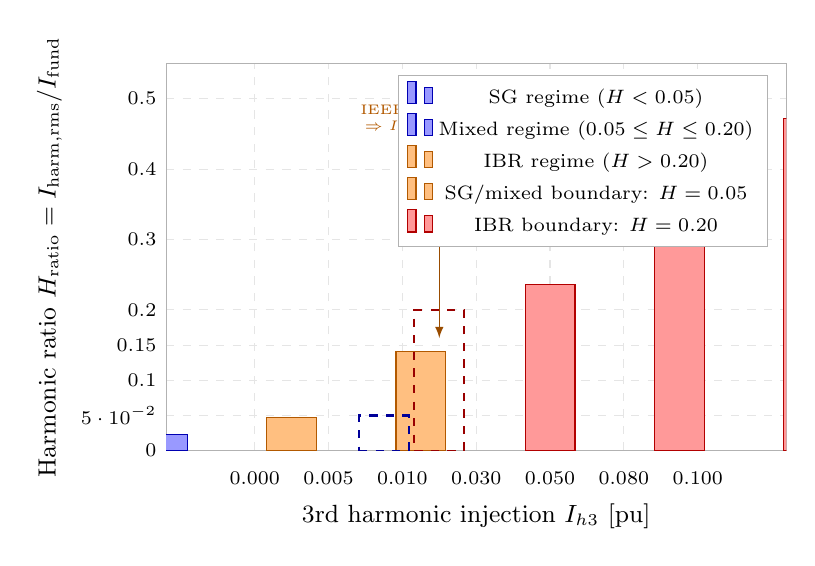
\begin{tikzpicture}
\begin{axis}[
  name        = hrax,
  ybar,
  bar width   = 18pt,
  width       = 0.78\textwidth,
  height      = 6.5cm,
  ylabel      = {Harmonic ratio $H_{\rm ratio} = I_{\rm harm,rms} / I_{\rm fund}$},
  ylabel style= {font=\small},
  xlabel      = {3rd harmonic injection $I_{h3}$ [pu]},
  xlabel style= {font=\small},
  ymin=0, ymax=0.55,
  ytick       = {0, 0.05, 0.10, 0.15, 0.20, 0.30, 0.40, 0.50},
  yticklabel style={font=\scriptsize},
  xtick       = {1, 2, 3, 4, 5, 6, 7},
  xticklabels = {0.000, 0.005, 0.010, 0.030, 0.050, 0.080, 0.100},
  xticklabel style={font=\scriptsize},
  enlarge x limits=0.10,
  legend style={at={(0.97,0.97)}, anchor=north east,
                font=\scriptsize, draw=gray!60},
  grid         = major,
  grid style   = {gray!20, dashed},
  tick style   = {draw=none},
  axis line style={gray!60},
]

% H_ratio values (I_fund_true=0.150, I_harm_rms = I_h3*sqrt(1^2+0.5^2+0.25^2)/sqrt(2))
% For harmonics (3,5,7) with amplitudes (1, 0.5, 0.25)×I_h3:
%   I_harm_rms = I_h3 × sqrt((1^2+0.5^2+0.25^2)/2) = I_h3 × sqrt(1.3125/2) ≈ I_h3 × 0.809
%   H_ratio = I_harm_rms / 0.150 ≈ I_h3 × 5.394

% Color by network type: SG=blue, mixed=orange, IBR=red
\addplot[fill=blue!40, draw=blue!70!black]
  coordinates {(1, 0.0000)};
\addplot[fill=blue!40, draw=blue!70!black]
  coordinates {(2, 0.0236)};
\addlegendentry{SG regime ($H < 0.05$)}

\addplot[fill=orange!50, draw=orange!70!black]
  coordinates {(3, 0.0472)};
\addplot[fill=orange!50, draw=orange!70!black]
  coordinates {(4, 0.1415)};
\addlegendentry{Mixed regime ($0.05 \leq H \leq 0.20$)}

\addplot[fill=red!40, draw=red!70!black]
  coordinates {(5, 0.2358)};
\addplot[fill=red!40, draw=red!70!black]
  coordinates {(6, 0.3773)};
\addplot[fill=red!40, draw=red!70!black]
  coordinates {(7, 0.4717)};
\addlegendentry{IBR regime ($H > 0.20$)}

% SG threshold line
\addplot[blue!60!black, thick, dashed, mark=none, domain=0.5:7.5, samples=2]
  ({x}, {0.05});
\addlegendentry{SG/mixed boundary: $H=0.05$}

% IBR threshold line
\addplot[red!60!black, thick, dashed, mark=none, domain=0.5:7.5, samples=2]
  ({x}, {0.20});
\addlegendentry{IBR boundary: $H=0.20$}

% IEEE 519 annotation
\node[font=\tiny, orange!70!black, align=center]
  at (axis cs:3.5, 0.47)
  {IEEE 519 THD 5\%\\$\Rightarrow I_{h3} \approx 0.035$\,pu};
\draw[-latex, orange!60!black, thin]
  (axis cs:3.5, 0.43) -- (axis cs:3.5, 0.16);

\end{axis}
\end{tikzpicture}
